\begin{frame}{Ejecucion de la Primer App en Android}
\begin{columns}
\begin{column}{0.8\textwidth}
\begin{itemize}
\item El dispositivo debe estar reconocido por Android y la compilación de la primera APP debe haber terminado. 
\item En la barra superior de Android Studio, presionar la flecha verde para instalar y ejecutar la app en el disposivito, 
\end{itemize}
\begin{block}{Demo \#00}
Muestra un TextView con el texto centrado "Hello World!"
\end{block}
\end{column}
\begin{column}{0.2\textwidth}
\begin{center}

 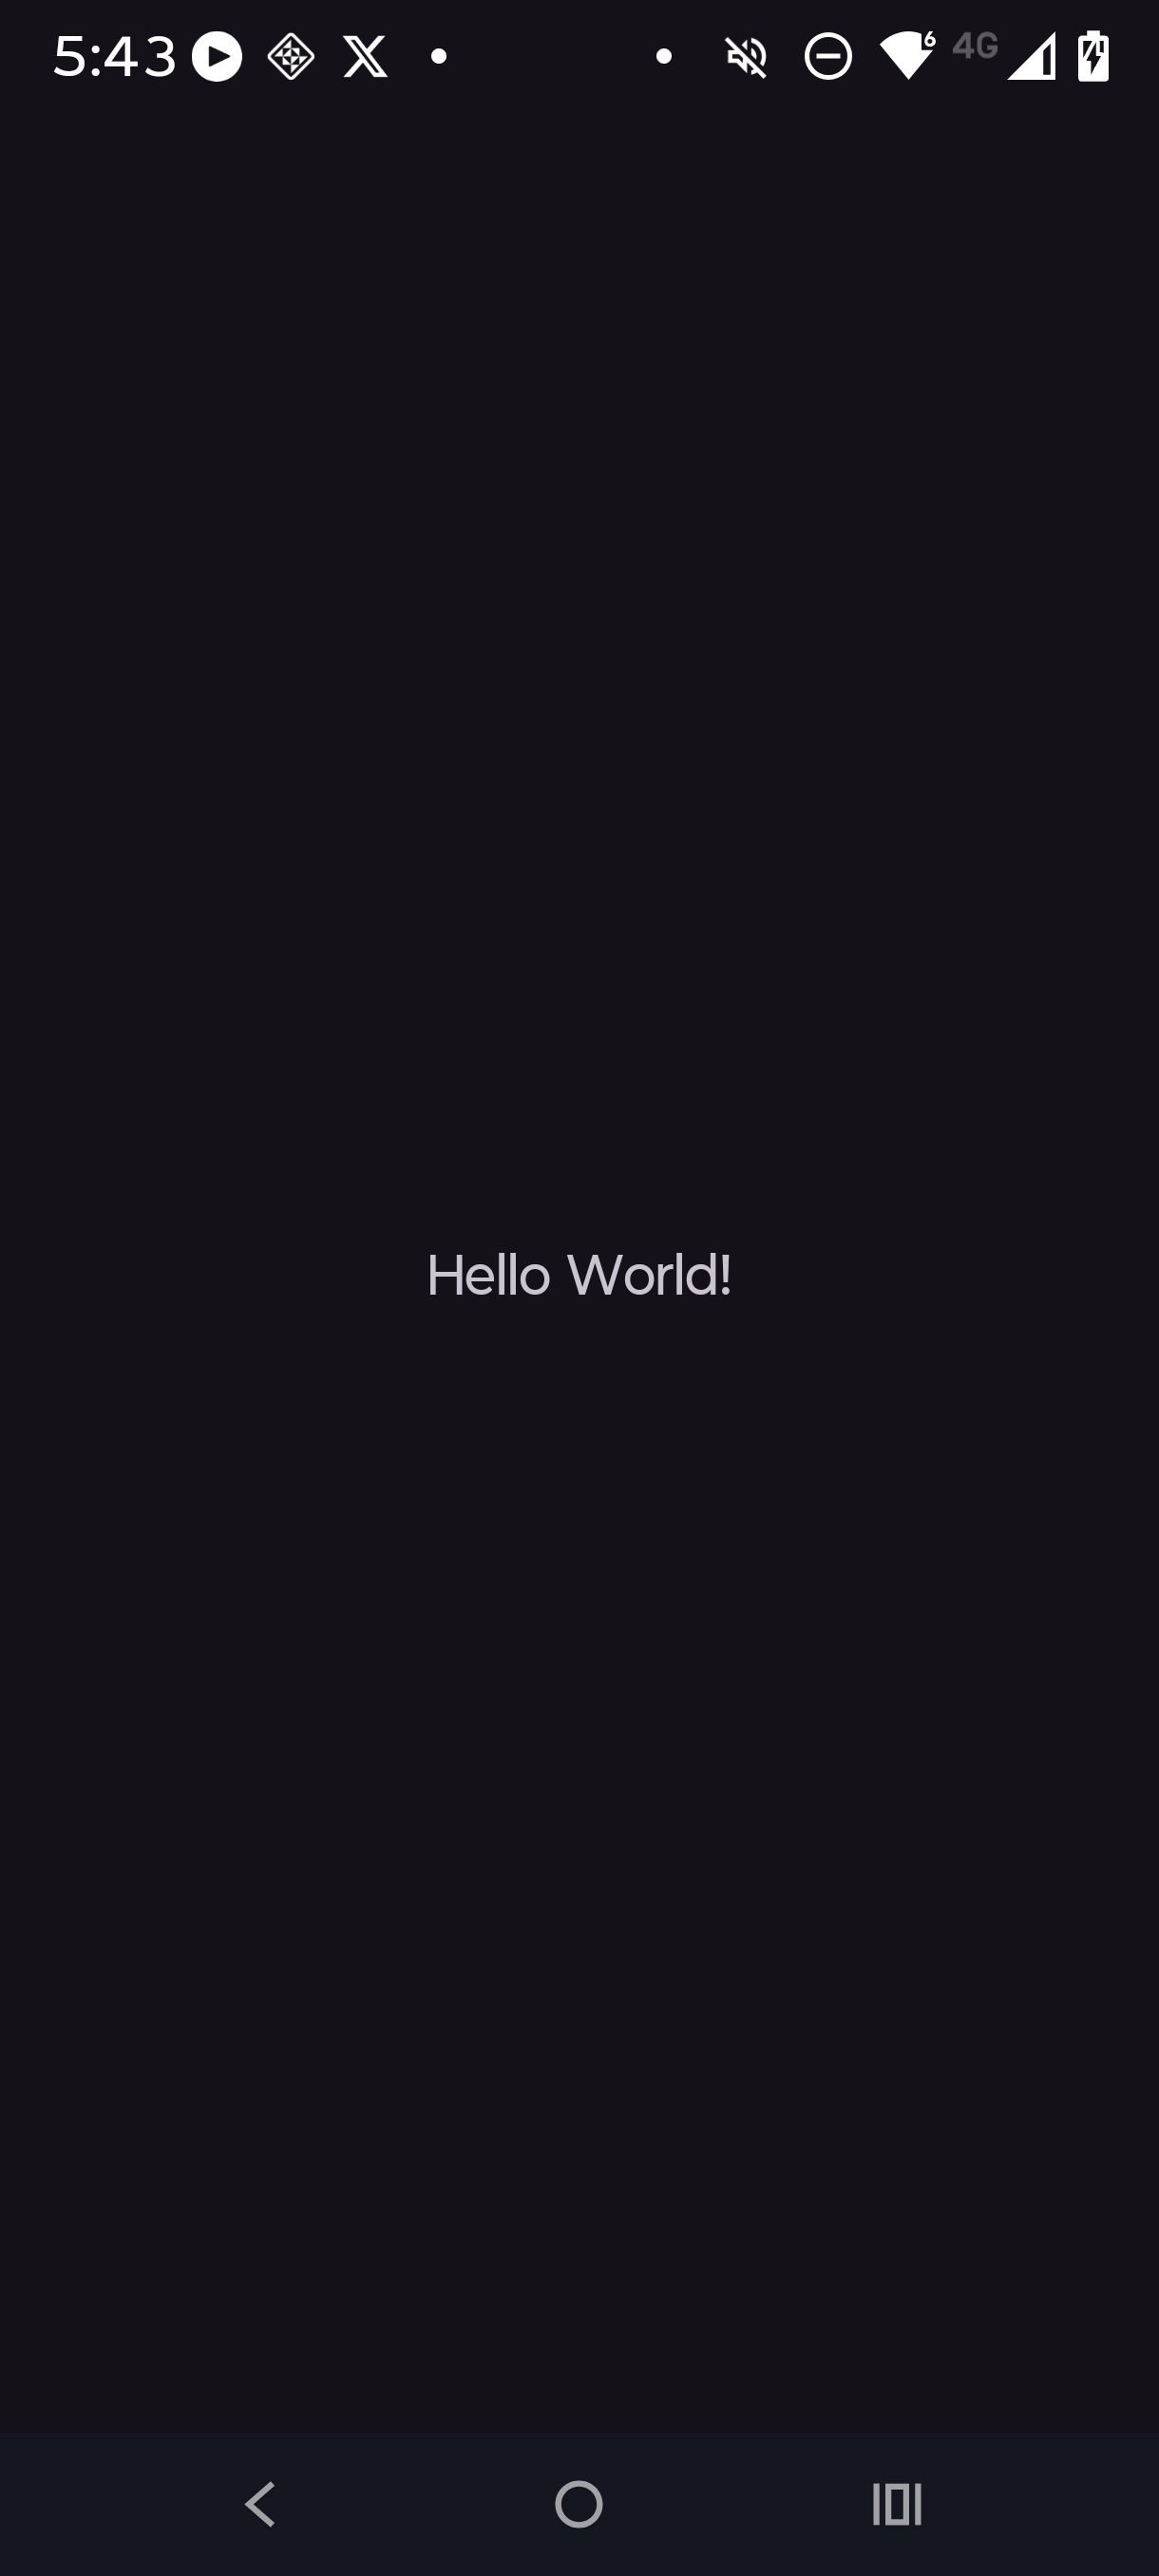
\includegraphics[width=0.98\textwidth]{02_TallerCBTis/figs/Demo00}
\end{center}
\end{column}
\end{columns}

\end{frame}


\begin{frame}[fragile]
\frametitle{Demo 01: Modificar el activity\_main.xml para aregar otro TextView}
\begin{columns}
\column{0.80\linewidth}
De los códigos fuentes en Github (como un archivo .zip), descomprimirlo y localizar los archivos mencionados a continuación:
\begin{itemize}
\item Copiar el archivo \textit{MainActivity\_Demo01.java} (dentro del Folder códigosJAVA) al mismo directorio donde esta el \textit{MainActivity.java}.
\item Copiar el archivo \textit{activity\_main\_demo01.xml} (dentro del Folder Carpeta\_layout) al mismo directorio donde esta el \textit{activity\_main.xml}
\item Modificar en el archivo AndroidManifest.xml la cadena \textit{.MainActivity} por \textit{.MainActivity\_Demo01}.
\end{itemize}

\begin{block}{Demo \#01}
Muestra un TextView con el texto centrado "Hello World!" (fuente verde, fondo rojo) 
\end{block}


\column{0.20\linewidth}

\begin{center}
 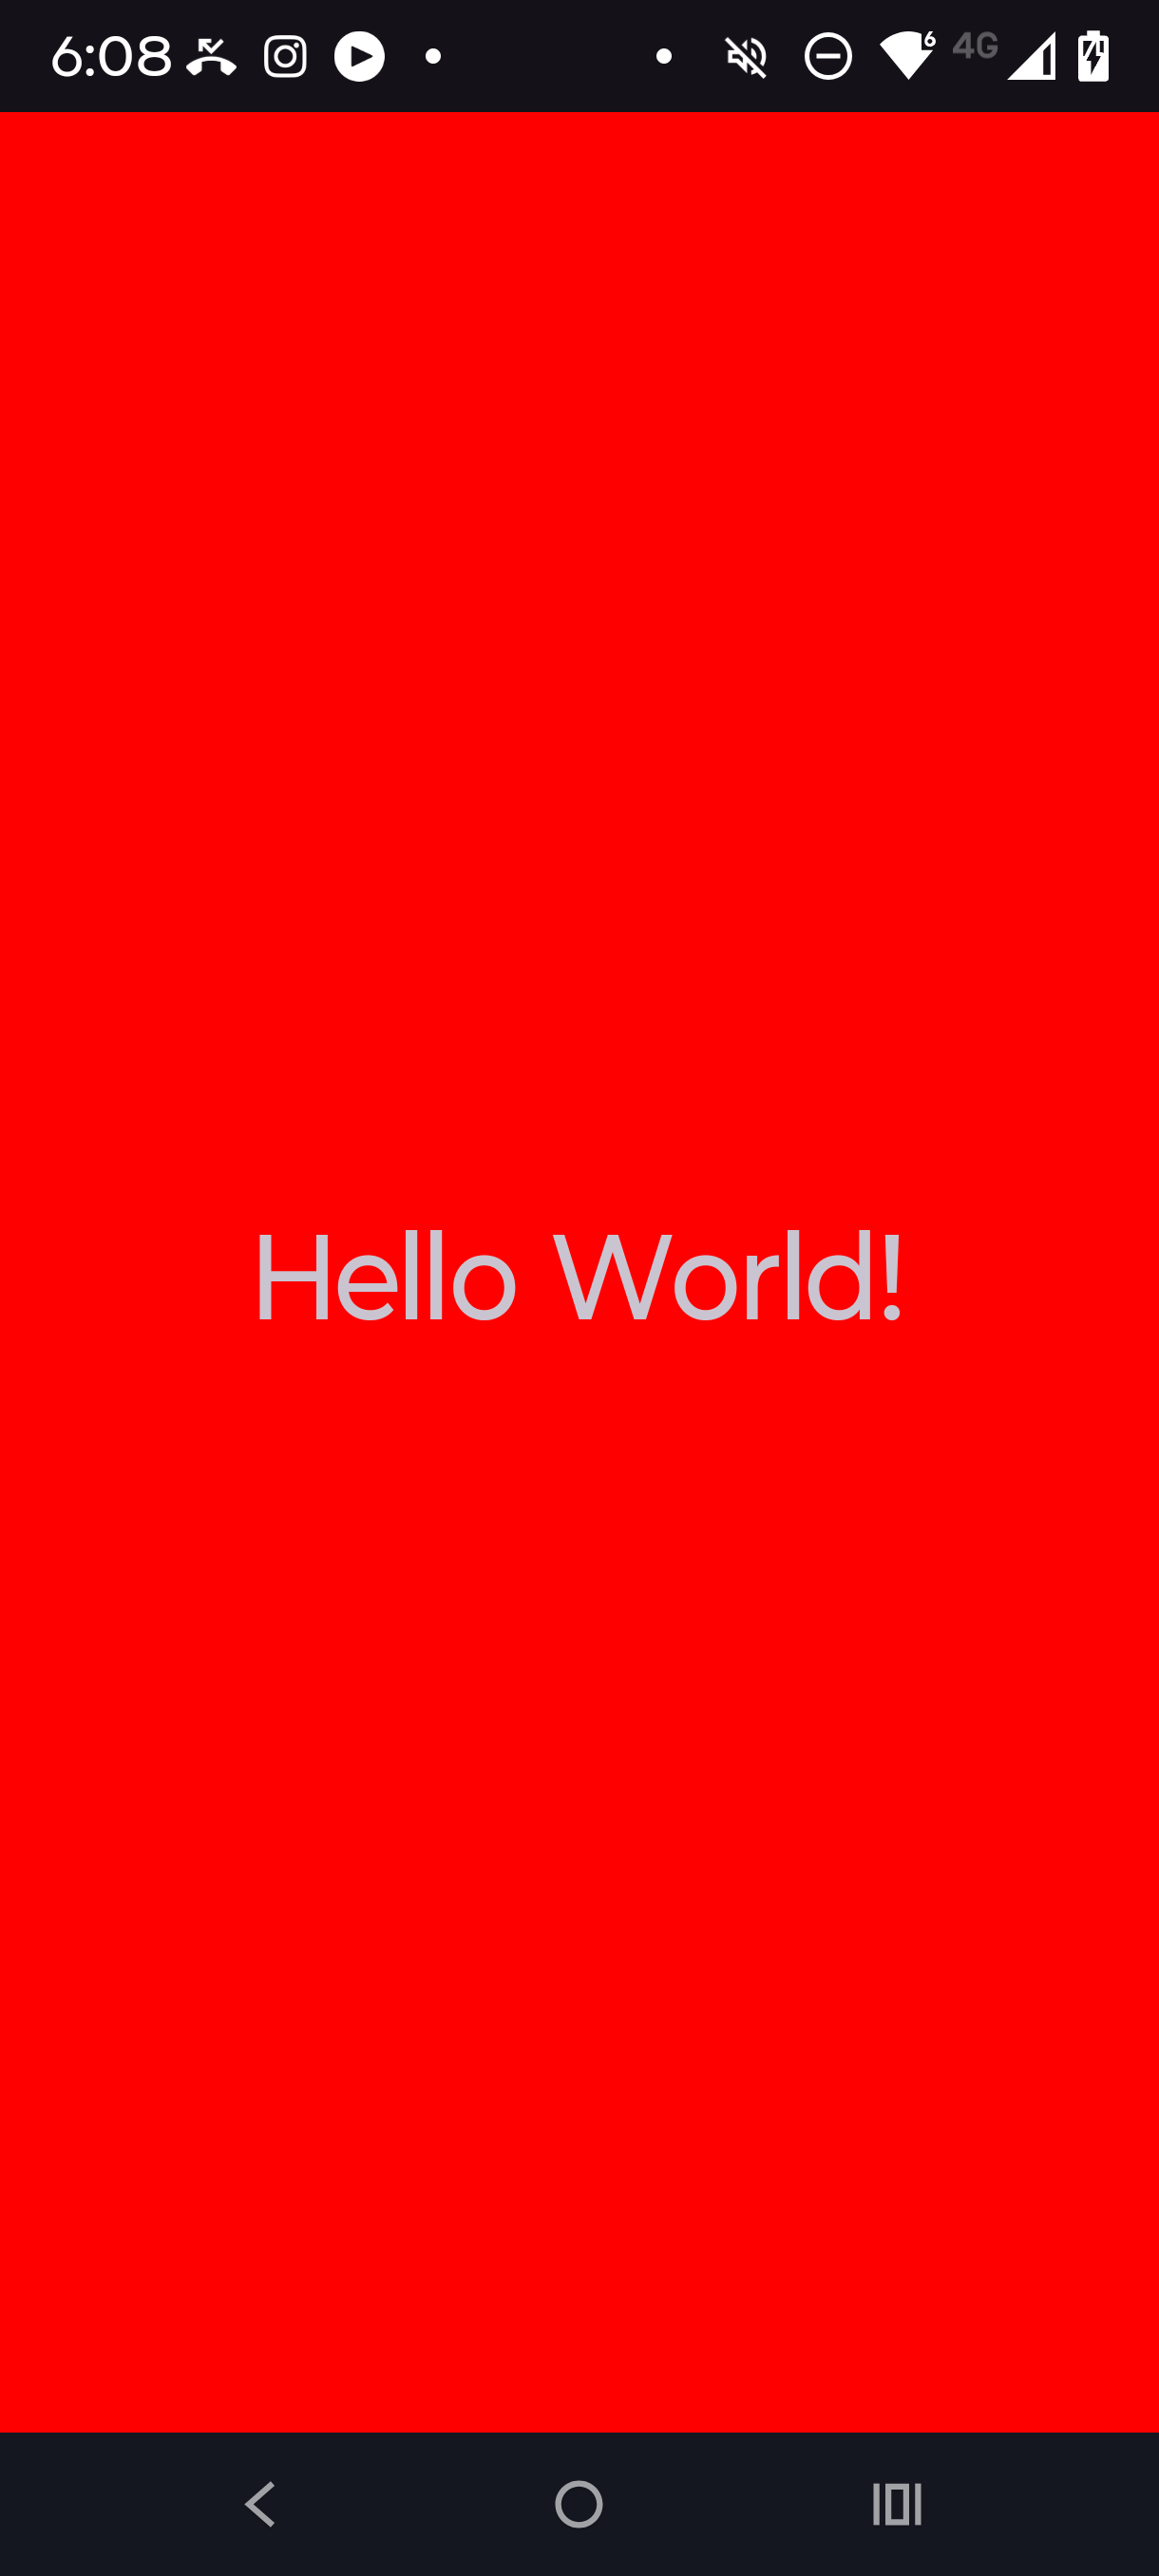
\includegraphics[width=0.98\textwidth]{02_TallerCBTis/figs/Demo01}
\end{center}

\end{columns}

\end{frame}


\begin{frame}{Modificaciones de Interés}

\begin{block}{Ejercicio \#01}
\begin{itemize}
\item Duplicar el TextView pero modificando el color de dichos componentes. 
\item Probar diferentes combinaciones del valor \textit{layout\_weight} en dichos componentes. 

\end{itemize}
\end{block}


\end{frame}

